\documentclass[11pt,a4paper]{article}
\usepackage[margin=2cm]{geometry}
\usepackage[T1]{fontenc}
\usepackage{lmodern}
\usepackage{xcolor}
\usepackage{graphicx}
\usepackage{titlesec}
\usepackage{enumitem}
\usepackage{booktabs}
\usepackage{tabularx}
\usepackage{fancyhdr}
\usepackage{float}
\usepackage[most]{tcolorbox}

\graphicspath{{figures/}}
\definecolor{lcpurple}{HTML}{6D3A8C}
\definecolor{lcteal}{HTML}{2F7F79}
\definecolor{lcpaper}{HTML}{F4EAD7}
\titleformat{\section}{\Large\bfseries\color{lcpurple}}{\thesection}{0.6em}{}
\titleformat{\subsection}{\large\bfseries\color{lcteal}}{}{0em}{}
\setlist{itemsep=2pt,topsep=4pt}
\pagestyle{fancy}\fancyhf{}\renewcommand{\headrulewidth}{0pt}
\fancyfoot[C]{\small Little Commanders --- rulebook draft v0.2 --- \thepage}
\setlength{\parindent}{0pt}\setlength{\parskip}{6pt}

% inline icon from the shared SVG set (design/icons.py)
\newcommand{\ic}[1]{\raisebox{-0.28em}{\includegraphics[height=1.25em]{#1.png}}}
\newcommand{\icbig}[1]{\includegraphics[height=2.2em]{#1.png}}
\newtcolorbox{tip}[1][]{colback=lcpaper,colframe=lcteal,boxrule=0.8pt,arc=2pt,left=6pt,right=6pt,top=4pt,bottom=4pt,#1}

\begin{document}

\begin{center}
{\Huge\bfseries\color{lcpurple} Little Commanders}\\[6pt]
{\large 2--6 players \quad $\cdot$ \quad 30--45 minutes \quad $\cdot$ \quad ages 8+}\\[2pt]
{\small Rulebook draft v0.2. Working title, art and numbers will change.}
\end{center}

\section{The Game in One Minute}
You are a kid commander with cute little \ic{bot} \textbf{Bots} and a few big \ic{mech} \textbf{Mechs}. Spread across the hex floor, hold tiles, and complete \ic{mission} \textbf{Missions} to earn \ic{vp} \textbf{Victory Points}. The first commander to reach the target wins.

\begin{tip}
\textbf{Two rules to remember.} (1) You spend \ic{credit} Credits to recruit, move and buy Missions. (2) Move onto an enemy tile with more strength than the defenders and they must go. Everything else is printed on your board, the tiles and the cards.
\end{tip}

\section{Icons}
The same pictures are used on tiles, cards, boards and in this book.
\begin{center}
\renewcommand{\arraystretch}{1.25}
\begin{tabular}{@{}c l @{\hspace{1.5em}} c l @{\hspace{1.5em}} c l@{}}
\icbig{credit} & Credit & \icbig{iron} & Iron & \icbig{crystal} & Crystal \\
\icbig{bot} & Bot (power 1) & \icbig{mech} & Mech (power 5) & \icbig{vp} & Victory Point \\
\icbig{extractor} & Extractor & \icbig{factory} & Factory & \icbig{tower} & Guard Tower \\
\icbig{dock} & Dock & \icbig{port} & Port & \icbig{mission} & Mission card \\
\icbig{move} & Move (1 per step) & \icbig{push} & Push & \icbig{kill} & Kill \\
\icbig{income} & Income & \icbig{trade} & Trade & \icbig{used} & Used this turn \\
\icbig{hex} & Tile & \icbig{centre} & Centre tile & \icbig{control} & Control a tile \\
\icbig{up} & Price goes up & \icbig{down} & Price goes down & \icbig{road} & Road \\
\end{tabular}
\end{center}

\section{Components}
\begin{itemize}
\item \textbf{Tiles:} 37 land tiles, 6 Home tiles, 12 Port tiles.
\item \textbf{Boards:} 6 Commander boards (Basic side and Advanced side), 1 Market board.
\item \textbf{Per commander:} 20 Bots, 6 Mechs, 5 Extractors, 5 Factories, 5 Guard Towers, 1 Dock.
\item \textbf{Tokens:} Iron, Crystal, Credit coins (1, 5, 10), price markers, VP markers.
\item \textbf{Cards:} 40 Missions (20 of Level 1, 20 of Level 2).
\end{itemize}

\section{Setup}
\begin{enumerate}
\item \textbf{Build the floor.} 2--3 players: 19 land tiles (centre and 2 rings). 4--6 players: 37 land tiles (centre and 3 rings). Shuffle the tiles of each ring and place them at random. Roads only connect where \emph{both} touching tiles show one.
\item \textbf{Ports.} Place 2 Port tiles per player around the outside. Each Port is joined by road to the 2 land tiles beside it.
\item \textbf{Homes.} Space the Home tiles evenly on the outer ring. Each player takes one, with a \ic{dock} Dock and a \ic{tower} Guard Tower, \ic{iron} \textbf{2 Iron} and \ic{bot} \textbf{3 Bots}.
\item \textbf{Missions.} Reveal 5 Missions. The deck is 10 random Level 1 cards with 10 random Level 2 cards below them.
\item \textbf{Market} (Advanced game). Put each price marker at random in its starting band: Iron 4--7, Bots 4--7, Crystal 8--14, Mechs 8--14.
\end{enumerate}
\begin{center}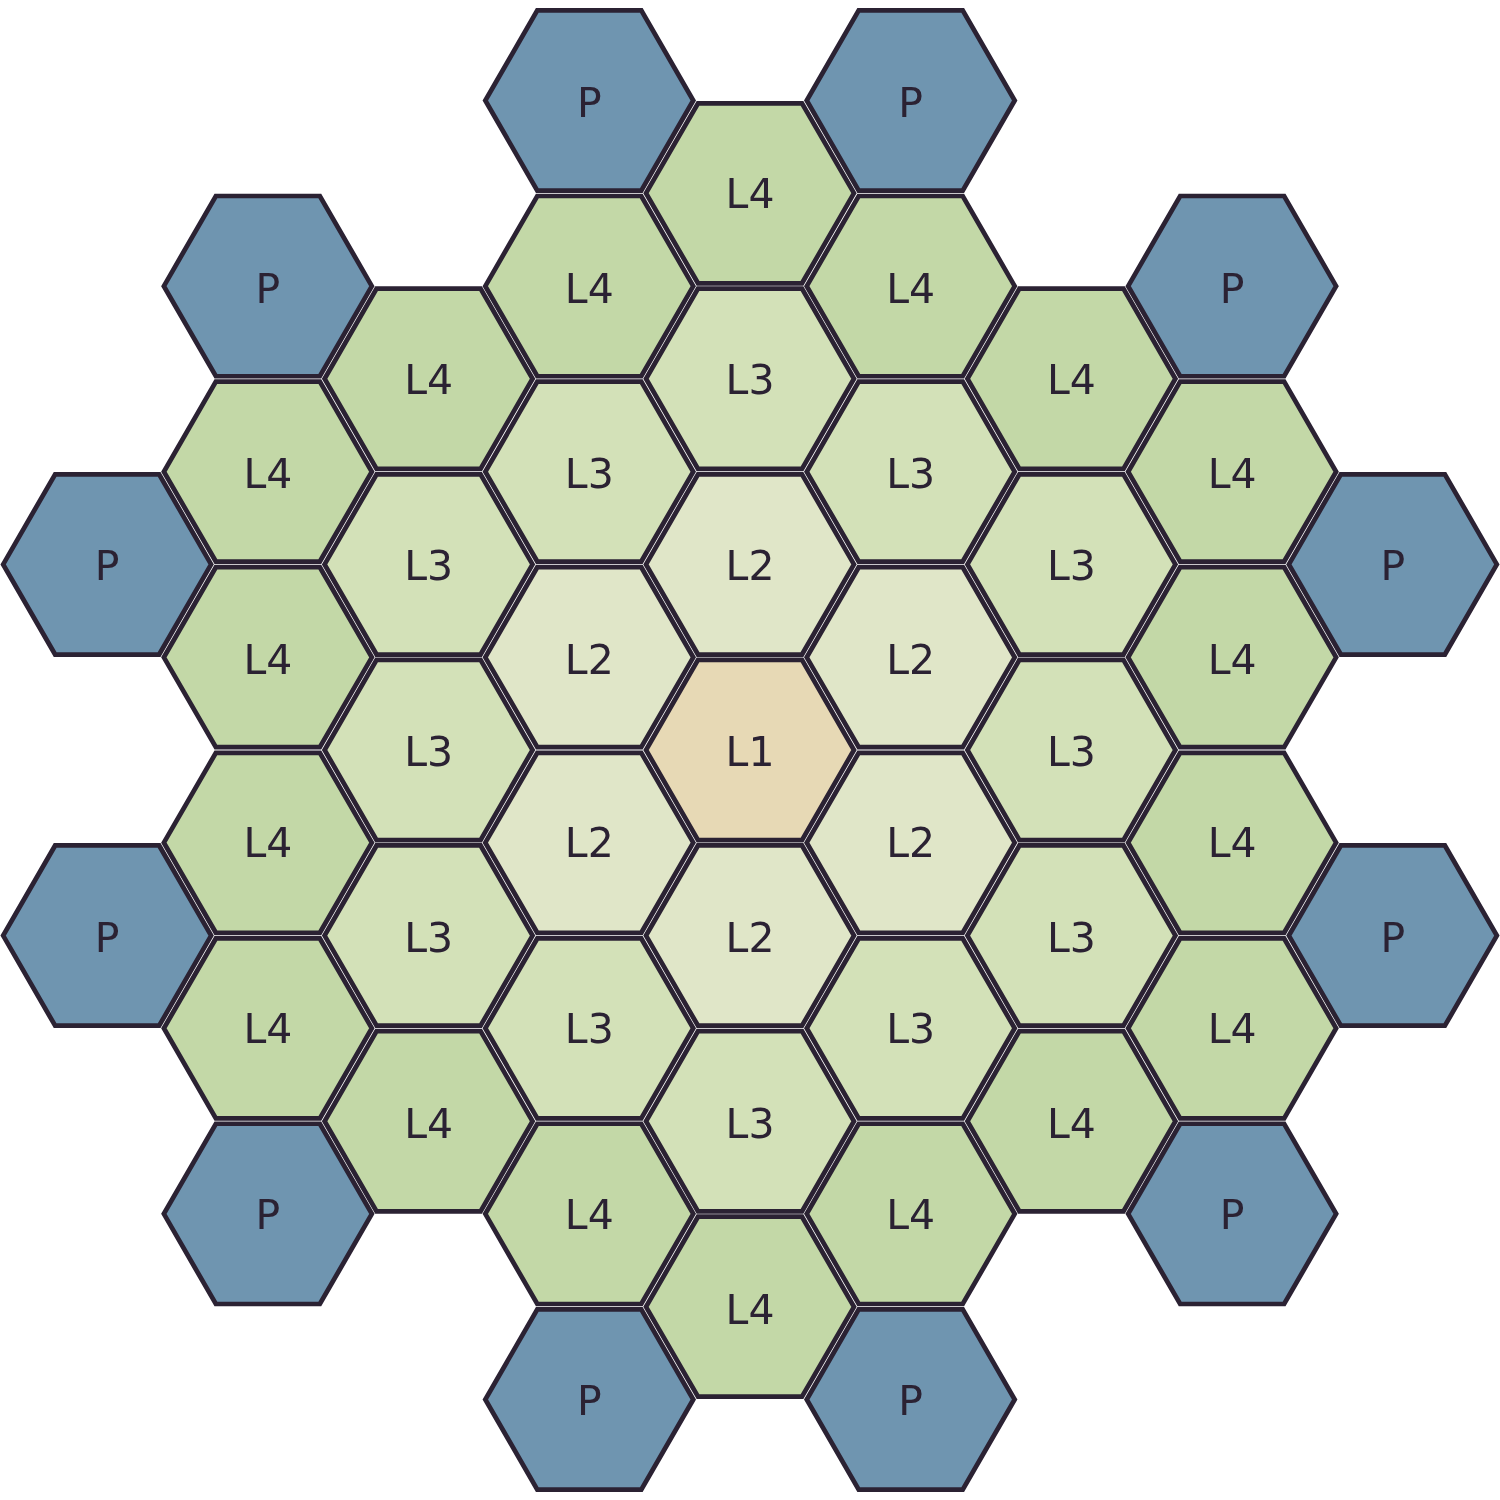
\includegraphics[width=0.55\textwidth]{board_layout.png}\\
{\small Four to six players: 37 land tiles and 12 Ports (shown schematically; L = land level, P = port).}\end{center}

\section{Reading a Tile}
\begin{center}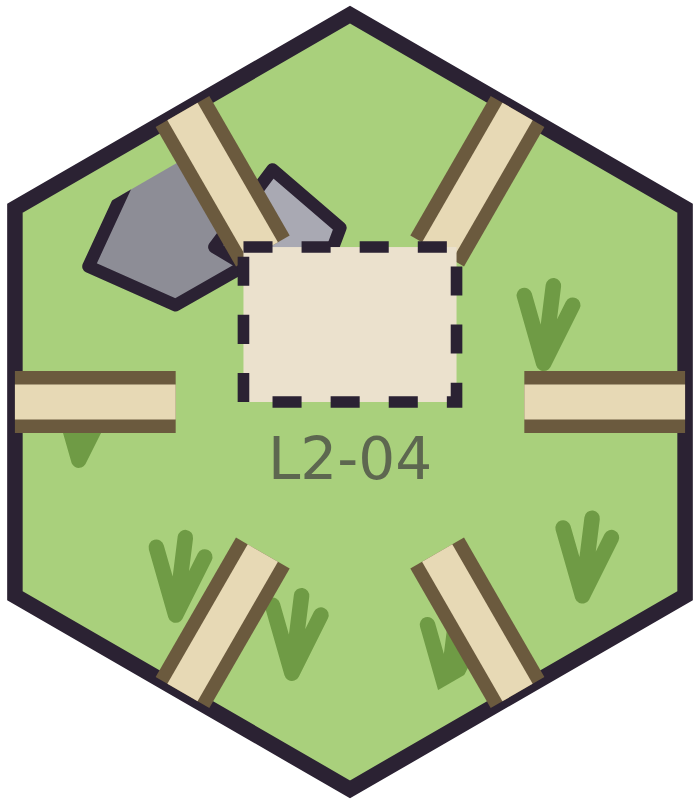
\includegraphics[width=0.38\textwidth]{land_L2_04.png}\end{center}
\begin{itemize}
\item \textbf{Ground:} green \ic{iron} Iron mine, blue \ic{crystal} Crystal deposit, or grey empty tile.
\item \textbf{Sockets:} 0, 1 or 2 square building areas where you may build.
\item \textbf{Roads:} a road on an edge means this tile connects there. A tiny broken stump means no road. Pieces only travel where \emph{both} tiles show a road.
\item \textbf{Code:} the small label (e.g.\ L2-04) is only for talking about tiles.
\end{itemize}
Tiles nearer the centre have more roads. The \ic{centre} centre has all six.

\section{Basic Game (draft)}
The Basic game uses only Bots, Credits and Missions. Use the Basic side of your board.
\begin{tcolorbox}[colback=white,colframe=lcteal,arc=2pt]
\textbf{Your turn}
\begin{enumerate}
\item \ic{income} \textbf{Income:} gain 1 Credit for every tile you hold.
\item \textbf{Spend Credits} in any order: \ic{bot} recruit a Bot on your home tile (2); \ic{move} move a piece one step along a road (1 per step); \ic{mission} buy a Mission (5, plus 1 for every Mission you have bought).
\item \ic{push} \textbf{Fight:} move onto an enemy tile. With more Bots than the defenders, they retreat. Otherwise yours go back.
\end{enumerate}
\textbf{Win} by being first to 3 \ic{vp} Victory Points. Use only Level 1 Missions.
\end{tcolorbox}

\clearpage
\section{Advanced Game}
Turn your board to the Advanced side. Everything in the Basic game is replaced by the rules below.

\subsection{Your Turn}
At the start of your turn gain \ic{income} \textbf{10 Credits} and take the coins off your buildings. Then do any of the following, in any order. End your turn when you are done. Your attacks are decided then.

\subsection{Control}
You \ic{control} \textbf{control} a tile while at least one of your pieces stands on it. Buildings and tokens on a tile belong to whoever controls it. Bots cannot be assigned to anything; they hold tiles and attack.

\subsection{Build and Make}
Spend iron that is standing on the tile on a free socket there. Build your first Extractor with your starting Iron.
\begin{center}
\renewcommand{\arraystretch}{1.3}
\begin{tabularx}{0.95\textwidth}{@{}c l X c@{}}
\ic{extractor} & Extractor & Once per turn, pay 1 Credit: take 1 token of the tile's resource. & 1 \ic{iron} \\
\ic{factory} & Factory & Once per turn, pay 1 Credit: 1 \ic{iron} becomes 2 \ic{bot}, or 1 \ic{iron} $+$ 1 \ic{crystal} becomes 1 \ic{mech}. & 2 \ic{iron} \\
\ic{tower} & Guard Tower & Makes the tile harder to push and kill. & 2 \ic{iron} \\
\end{tabularx}
\end{center}
When a building or trading post works, put a \ic{used} coin on it. Take the coins back at the start of your turn. You may sell a building: it returns to your board and you get its cost minus 1 Iron on the tile.

\subsection{Move}
\ic{move} Every step costs 1 Credit per piece. You may move a piece several steps in a turn, paying for each. Pieces follow open roads and cannot pass through enemy pieces. Put a coin under a piece that has moved this turn.

\subsection{Trade}
\ic{trade} Stand on a tile with your \ic{dock} Dock or on a \ic{port} Port. Each post trades once per turn: pay 1 Credit, then choose one good and buy or sell any number of it at the current price.
\begin{itemize}
\item \textbf{Home Dock:} Iron and Bots, at the normal price.
\item \textbf{Port:} one good is 2 cheaper to buy, or pays 3 more when sold.
\item Afterwards the price moves one step for every item traded: \ic{up} when you buy, \ic{down} when you sell. A step is 1 Credit for Iron and Bots and 2 for Crystal and Mechs.
\item Ranges: Iron 1--10, Bots 1--10, Crystal 2--20, Mechs 2--20.
\end{itemize}

\subsection{Missions}
\begin{minipage}{0.62\textwidth}
Pay \ic{credit} \textbf{5 Credits} to buy a face-up Mission, plus 1 for every Mission you have bought. You may buy one per turn. If you meet it \emph{at that moment}, you score its \ic{vp} (1 for Level 1, 2 for Level 2). If not, the Credits are lost. A completed card is replaced from the deck.
\end{minipage}\hfill
\begin{minipage}{0.34\textwidth}
\includegraphics[width=\textwidth]{L1_12_land-grab-3.png}\end{minipage}

\subsection{Combat}
Move onto an enemy tile to attack it. Attackers walk in; the attack is decided when you end your turn.
\begin{itemize}
\item \ic{bot} Bot power 1. \ic{mech} Mech power 5. Add up each side's power.
\item \ic{push} \textbf{Push:} attackers have at least $2\times$ the defenders' power. The defenders retreat; the defending player chooses where each piece goes.
\item \ic{kill} \textbf{Kill:} at least $3\times$. The defenders are removed.
\item \ic{tower} Each Guard Tower on the tile adds 1 to both multipliers ($2\to3$, $3\to4$, \dots).
\item Not enough? The attack \textbf{fails} and the attackers return to where they came from.
\end{itemize}

\subsection{Winning}
Be first to \textbf{5} \ic{vp} Victory Points. Points come only from Missions.

\section{Factions}
Each commander has a colour and a different silhouette, so the game also works without colour vision. Faction powers are an optional extra still being designed.

\section{Your Board}
\begin{figure}[H]\centering
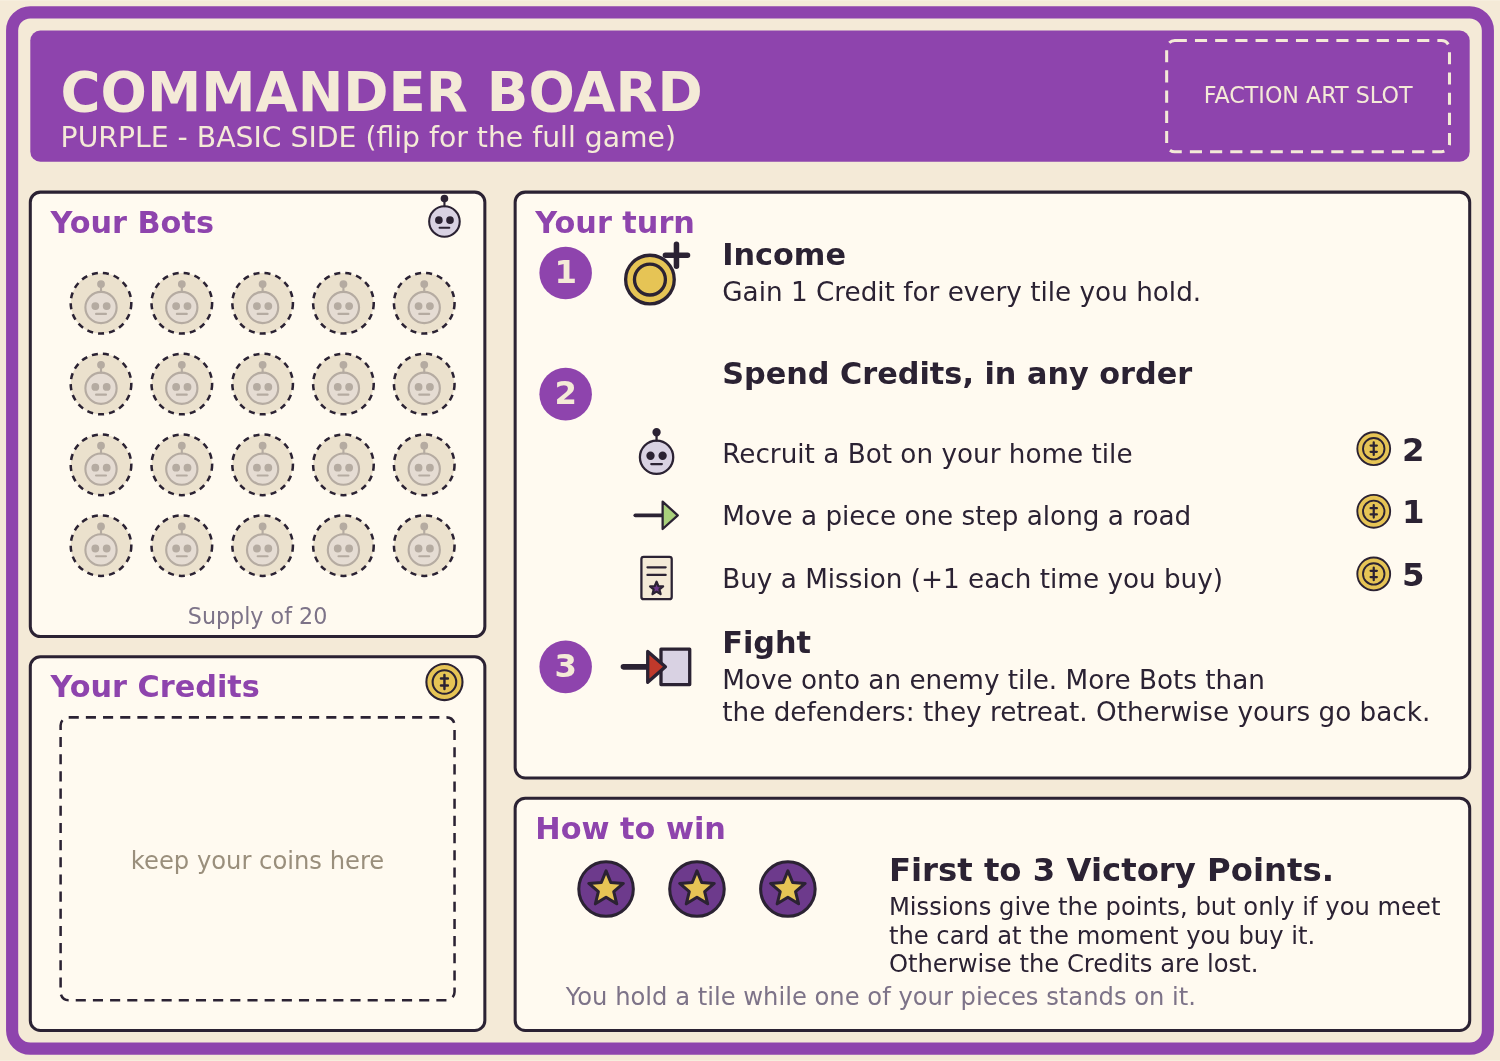
\includegraphics[width=0.92\textwidth]{player_board_purple_basic.png}\\[6pt]
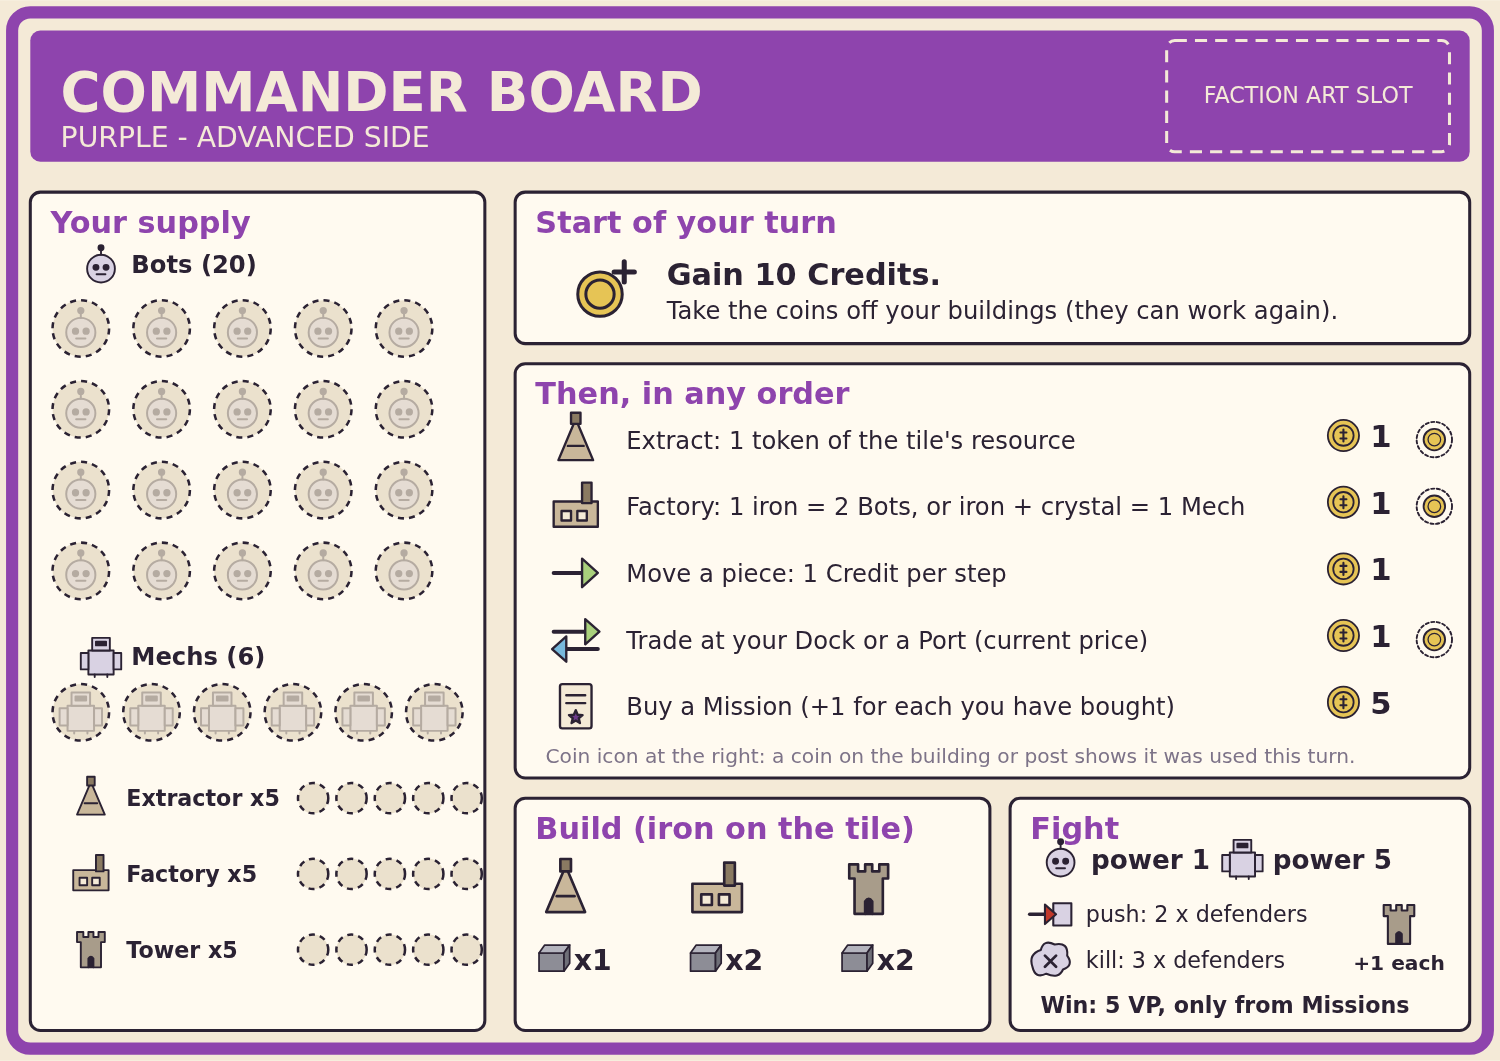
\includegraphics[width=0.92\textwidth]{player_board_purple_advanced.png}
\caption{Basic side (front) and Advanced side (back).}
\end{figure}

\section{Draft Notes}
\begin{itemize}
\item Basic game numbers (2 Credits per Bot, 3 VP) are untested.
\item The used-coin rule and one trade per post per turn are agreed but not yet in the BGA version.
\item Movement was triangular (1, 3, 6, 10 per piece); it is now linear. See \texttt{DESIGN\_NOTES.md}.
\end{itemize}

\end{document}
